\subsubsection{January 13}

\subsubsection*{True (\trueIcon) false (\falseIcon) questions}

\begin{enumerate}
    \item \trueIcon \: SANs are primarily used for block-level access to data, while NAS devices provide file-level access.
    \item \trueIcon \: RAID can be used with both hardware and software implementations.
    \item \falseIcon \: GPUs (Graphics Processing Units) are primarily used in datacenters for accelerating graphical applications and gaming.
    \item \falseIcon \: Cloud computing applications do not require any server to run.
    \item \falseIcon \: Availability zones within a Compute Region can have a roundtrip time larger than few milliseconds.
    \item \trueIcon \: Edge computing is a distributed computing paradigm that brings computation and data storage closer to the location where it is needed.
    \item \falseIcon \: The power consumption of an average datacenter is in the order of a few GigaWatts.
    \item \falseIcon \: Leaf-spine topologies are more suitable for small-scale datacenter deployments with limited server connections.
    \item \trueIcon \: Warehouse-scale computers are typically composed of a large set of homogeneous servers.
    \item \trueIcon \: Virtualization can help simplify IT management by reducing the number of physical machines that need to be managed.
\end{enumerate}

\newpage

\subsubsection*{Exercises}

\begin{enumerate}
    \setcounter{enumi}{10}

    \item A scientific computation that needs to be carried out within the PoliMi data center uses a server composed of 2 CPUs and 4 GPUs. Knowing that:
    \begin{itemize}
        \item The computation takes 8 days to complete,
        \item The computation requires at least one CPU and all GPUs within the server to be operational to complete successfully;
        \item $\text{MTTF}_{\text{CPU}} = 180$ days and $\text{MTTF}_\text{GPU} = 120$ days.
    \end{itemize}
    How many parallel instances of the computation must be launched to ensure a probability higher than 98\% that at least one computation produces results successfully? Notes: (i) Use at least 4 decimal places for all intermediate calculations. (ii) All other components of the server can be considered ideal.

    \emph{\textcolor{Green3}{\textbf{Answer:}}} Each instance has some chance of \emph{surviving} 8 days:
    \begin{itemize}
        \item If we run $n$ instances, the probability that \emph{all fail} is $P_{\text{fail}}^n$.
        \item So: $P_{\text{success, total}} = 1 - P_{\text{fail}}^n$.
        \item Require: $1 - P_{\text{fail}}^n \ge 0.98 \quad \Rightarrow \quad 1 - \left(P_{\text{fail 1 job}}\right)^{n} \ge 0.98$
    \end{itemize}
    We can retrieve the RBD from the system:
    \begin{center}
        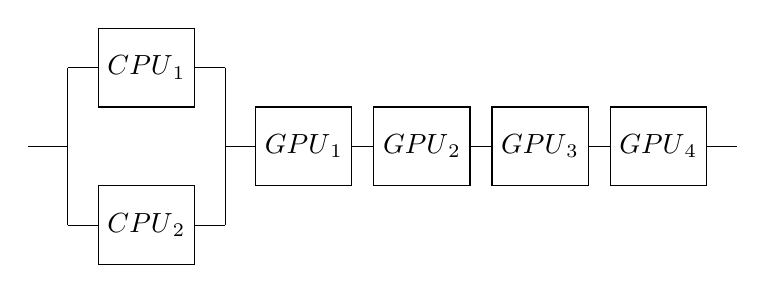
\begin{tikzpicture}[node distance=2cm]
            \draw (0,0) -- (0.5,0);

            \draw (0.5,0) -- (0.5,1);
            \draw (0.5,0) -- (0.5,-1);

            \node[
                draw,
                minimum width=1cm,
                minimum height=1cm,
                name=cpu1
            ] at (1.5,1) {$\text{CPU}_1$};
            \node[
                draw,
                minimum width=1cm,
                minimum height=1cm,
                name=cpu2
            ] at (1.5,-1) {$\text{CPU}_2$};

            \draw (0.5,1) -- (cpu1);
            \draw (0.5,-1) -- (cpu2);

            \draw (cpu1) -- (2.5,1);
            \draw (cpu2) -- (2.5,-1);

            \draw (2.5,1) -- (2.5,0);
            \draw (2.5,-1) -- (2.5,0);

            \node[
                draw,
                minimum width=1cm,
                minimum height=1cm,
                name=gpu1
            ] at (3.5,0) {$\text{GPU}_1$};

            \draw (2.5,0) -- (gpu1);

            \node[
                draw,
                minimum width=1cm,
                minimum height=1cm,
                name=gpu2
            ] at (5,0) {$\text{GPU}_2$};

            \draw (gpu1) -- (gpu2);

            \node[
                draw,
                minimum width=1cm,
                minimum height=1cm,
                name=gpu3
            ] at (6.5,0) {$\text{GPU}_3$};

            \draw (gpu2) -- (gpu3);

            \node[
                draw,
                minimum width=1cm,
                minimum height=1cm,
                name=gpu4
            ] at (8,0) {$\text{GPU}_4$};

            \draw (gpu3) -- (gpu4);

            \draw (gpu4) -- (9,0);
        \end{tikzpicture}
    \end{center}
    \begin{enumerate}
        \item \textbf{Probability CPUs survive}. A single CPU survives 8 days with probability (see page \pageref{eq: failure rate}):
        \begin{equation*}
            P_{\text{CPU, survive}} = R(t) = e^{-t \lambda} = e^{-\frac{8}{180}}
        \end{equation*}
        Where $\lambda = \dfrac{1}{\text{MTTF}}$. So, the probability that the system fails when the last component fails is (see page \pageref{eq: system fails when the last component fails - parallel}), then the probability that everything works:
        \begin{equation*}
            \begin{array}{rcl}
                R_S(t) &=& 1 - \displaystyle\prod_{i=1}^{n = 2} \left[1 - e^{-\frac{8}{180}}\right] \\ [1.3em]
                %
                &=& 1 - \left(1 - e^{-\frac{8}{180}}\right)^{2} \\ [.8em]
                %
                &=& 1 - \left(1 - 0.956528739\right)^{2} \\ [.3em]
                %
                &=& 1 - \left(0.043471261\right)^{2} \\ [.3em]
                %
                &=& 1 - 0.001889751 \\ [.3em]
                %
                &=& 0.998110249
            \end{array}
        \end{equation*}

        \newpage

        \item \textbf{Probability GPUs survive}. GPUs have the survival probability:
        \begin{equation*}
            P_{\text{GPU, survive}} = R(t) = e^{-t \lambda} = e^{-\frac{8}{120}}
        \end{equation*}
        So, the system failure is determined by the failure of the first component (see page \pageref{eq: system fails when the last component fails - sequential}), then the probability that everything works:
        \begin{equation*}
            \begin{array}{rcl}
                R_S(t) &=& \displaystyle\prod_{i=1}^{n=4} e^{-\frac{8}{120}} \\ [1.3em]
                %
                &=& \left(e^{-\frac{8}{120}}\right)^{4} \\ [.8em]
                %
                &=& \left(0.935506985\right)^{4} \\ [.3em]
                %
                &=& 0.765928338
            \end{array}
        \end{equation*}

        \item \textbf{Probability that one job fail}. We calculate the probability of a system failure by starting with the system's overall reliability.:
        \begin{equation*}
            \begin{array}{rcl}
                P_{\text{fail, 1 job}} &=& 1 - \left(0.998110249 \cdot 0.765928338\right) \\ [.3em]
                &=& 1 - 0.764480924 \\ [.3em]
                &=& 0.235519076
            \end{array}
        \end{equation*}

        \item \textbf{Calculate the number of parallel instances}. Now that we have the probability of one job failing, we can substitute this value into the requirements formula to find the $n$ variable:
        \begin{equation*}
            \begin{array}{rcl}
                1 - P_{\text{fail}}^n &\ge& 0.98 \\ [.5em]
                1 - \left(P_{\text{fail 1 job}}\right)^{n} &\ge& 0.98 \\ [.5em]
                - \left(0.235519076\right)^{n} &\ge& 0.98 - 1 \\ [.5em]
                \left(0.235519076\right)^{n} &\le& 0.02 \\ [.5em]
                \ln\left(\left(0.235519076\right)^{n}\right) &\le& \ln\left(0.02\right) \\ [.5em]
                n \cdot \ln\left(0.235519076\right) &\le& \ln\left(0.02\right) \\ [.5em]
                &\downarrow& \le \text{ flips because } \ln\left(0.235519076\right) < 0 \\ [.5em]
                n &\ge& \dfrac{
                    \ln\left(0.02\right)
                }{
                    \ln\left(0.235519076\right)
                } \\ [1.3em]
                n &\ge& \dfrac{
                    -3.912023005
                }{
                    -1.445963367
                } \\ [1.3em]
                n &\ge& 2.705478641
            \end{array}
        \end{equation*}
        Therefore, $n$ must be greater than $2.71$ to achieve a reliability greater than 98\%. We round up to $n = 3$ because we are talking about real-world components.
    \end{enumerate}

    \newpage

    \item If the time required to recover and replace a component of the server described in the previous exercise (whether it is a CPU or a GPU) is equal to 24 days, what is the total availability of the server? Notes: (i) Use at least 5 decimal places for all intermediate calculations. (ii) All other components of the server can be considered ideal.
    
    \textcolor{Green3}{\textbf{\emph{Answer:}}} The exercise provides the Mean Time To Repair (MTTR), which is 24 days. With the help of the Reliability Block Diagram (RBD), we can easily determine which availability formula to use:
    \begin{itemize}
        \item \textbf{Availability of each CPU component} (see page \pageref{eq: Availability}):
        \begin{equation*}
            A_{\text{CPU}} = \dfrac{\text{MTTF}}{\text{MTTF} + \text{MTTR}} = \dfrac{180}{180+24} = 0.882352941
        \end{equation*}
        
        \item \textbf{Availability of each GPU component} (see page \pageref{eq: Availability}):
        \begin{equation*}
            A_{\text{GPU}} = \dfrac{\text{MTTF}}{\text{MTTF} + \text{MTTR}} = \dfrac{120}{120+24} = 0.833333333
        \end{equation*}

        \item \textbf{Availability CPU (parallel) group} (see page \pageref{eq: Availability of Parallel System - Simplified}):
        \begin{equation*}
            \begin{array}{rcl}
                A_{\text{CPUs}} &=& 1 - \left(1 - A_{\text{CPU}}\right)^{n} \\ [.5em]
                &=& 1 - \left(1 - 0.882352941\right)^{2} \\ [.5em]
                &=& 1 - \left(0.117647059\right)^{2} \\ [.5em]
                &=& 1 - 0.01384083 \\ [.5em]
                &=& 0.98615917
            \end{array}
        \end{equation*}

        \item \textbf{Availability GPU (series) group} (see page \pageref{eq: Availability of Series System - Simplified}):
        \begin{equation*}
            \begin{array}{rcl}
                A_{\text{GPUs}} &=& A_{\text{GPU}}^{n} \\ [.5em]
                &=& \left(0.833333333\right)^{4} \\ [.5em]
                &=& 0.482253086
            \end{array}
        \end{equation*}

        \item \textbf{Overall System Availability}:
        \begin{equation*}
            A_{\text{system}} = A_{\text{CPUs}} \cdot A_{\text{GPUs}} = 0.98615917 \cdot 0.482253086 = \mathbf{0.47557}8303
        \end{equation*}

        \item \textbf{Availability if we use 3 parallel instances}. The previous availability was achieved with a single server instance. If we follow the previous solution's suggestion and run 3 instances of the same server to achieve 98\% reliability, the system's availability will be (use parallel formula, see page \pageref{eq: Availability of Parallel System - Simplified}):
        \begin{equation*}
            \begin{array}{rcl}
                A_{\text{system with 3 instances}} &=& 1 - \left(1 - A_{\text{system}}\right)^{n} \\ [.5em]
                &=& 1 - \left(1 - 0.475578303\right)^{3} \\ [.5em]
                &=& 1 - \left(0.524421697\right)^{3} \\ [.5em]
                &=& 1 - 0.144225467 \\ [.5em]
                &=& \mathbf{0.85577}4533
            \end{array}
        \end{equation*}
    \end{itemize}

    \item A company is planning to use a RAID 5 array composed of 8 disks for critical data storage. The desired Mean Time To Failure for the entire RAID system ($\text{MTTF}_{\text{RAID5}}$) is 16 years. Each disk in the array has a MTTF disk equal to 500 days. What should be the MTTR required \emph{in hours} to meet the target RAID $\text{MTTF}_{\text{RAID5}}$ .
    
    \textcolor{Green3}{\textbf{\emph{Answer:}}} We know that the MTTF of the RAID 5 is (see page \pageref{eq: RAID 5 - MTTF}):
    \begin{equation*}
        \text{MTTF}_{\text{RAID5}} = \dfrac{
            \text{MTTF}_\text{disk}^{2}
        }{
            G \cdot \left(G-1\right) \cdot \text{MTTR}
        }
    \end{equation*}
    We can substitute the known values into the formula (where 16 years are 5840 days):
    \begin{equation*}
        \begin{array}{rcl}
            \text{MTTF}_{\text{RAID5}} &=& \dfrac{
                \text{MTTF}_\text{disk}^{2}
            }{
                G \cdot \left(G-1\right) \cdot \text{MTTR}
            } \\ [1.3em]
            %
            5840 &=& \dfrac{
                \left(500\right)^{2}
            }{
                8 \cdot \left(8-1\right) \cdot \text{MTTR}
            } \\ [1.3em]
            %
            5840 &=& \dfrac{
                250'000
            }{
                56 \cdot \text{MTTR}
            } \\ [1.3em]
            %
            5840 \cdot \text{MTTR} &=& \dfrac{
                250'000
            }{
                56 \cdot \cancel{\text{MTTR}}
            } \cdot \cancel{\text{MTTR}} \\ [1.3em]
            %
            \dfrac{1}{\cancel{5840}} \cdot \cancel{5840} \cdot \text{MTTR} &=& \dfrac{250'000}{56} \cdot \dfrac{1}{5840} \\ [1.3em]
            %
            \text{MTTR} &=& \dfrac{250'000}{327'040} \\ [1.3em]
            %
            \text{MTTR} &=& \mathbf{0.7644}32485 \, \text{days} \\ [.3em]
            %
            \text{MTTR} &=& 0.764432485 \text{ days} \cdot 24 \text{ hours} \\ [.3em]
            %
            \text{MTTR} &=& \mathbf{18.346}379648 \text{ hours}
        \end{array}
    \end{equation*}

    \newpage

    \item Consider a system composed of three stations: the CPU that is characterized by $V_{\text{CPU}} = 100$ visits and an average service time of $S_{\text{CPU}} =10$ms; the disk, characterized by a throughput of 12 IOPS, and a demand of $D_{\text{DISK}} =150$ms; and the GPU whose demand is $D_\text{GPU} = 40$s and the number of visits $V_{\text{GPU}} =10$. Finally, the system throughput is $X=20$ jobs/min while the response time when there are $N = 20$ end-users in the system is $R = 55$s. Compute the CPU demand and the GPU throughput. Write in the answer sheet: $D_\text{CPU} = \dots$; $X_\text{GPU} = \dots$.
    
    \textcolor{Green3}{\textbf{\emph{Answer:}}} First, we clarify the data we have.
    \begin{itemize}
        \item CPU:
        \begin{itemize}
            \item $V_{\text{CPU}} = 100$ visits
            \item $S_{\text{CPU}} =10$ms
        \end{itemize}
        \item Disk:
        \begin{itemize}
            \item Throughput of 12 IOPS
            \item $D_{\text{DISK}} =150$ms
        \end{itemize}
        \item GPU:
        \begin{itemize}
            \item $D_\text{GPU} = 40$s
            \item $V_{\text{GPU}} = 10$ visits
        \end{itemize}
        \item System:
        \begin{itemize}
            \item $X=20$ jobs/min
            \item If $N = 20$ end-users, then $R = 55$s
        \end{itemize}
    \end{itemize}
    The \textbf{CPU demand} is (see page \pageref{eq: Service Demand}):
    \begin{equation*}
        D_{\text{CPU}} = S_{\text{CPU}} \cdot V_{\text{CPU}} = 10 \cdot 100 = 1000 \, \text{ms} = \mathbf{1} \, \textbf{sec}
    \end{equation*}
    The \textbf{GPU throughput} is (see the Forced Flow Law, page \pageref{paragraph: Forced Flow Law}):
    \begin{equation*}
        X_{\text{GPU}} = V_{\text{GPU}} \cdot X = 10 \cdot 20 \,\text{jobs/sec} = \mathbf{200} \,\textbf{GPU ops/min}
    \end{equation*}

    \item Considering the system described in Question 14, what is the users' think time Z?
    
    \textcolor{Green3}{\textbf{\emph{Answer:}}} We use the Interactive Response Time Law (see page \pageref{paragraph: Interactive Response Time Law}):
    \begin{equation*}
        \begin{array}{rcl}
            R &=& \dfrac{N}{X} - Z \\ [1.3em]
            55 \, \text{sec} &=& \dfrac{20}{\left(20 \div 60\right) \,\text{jobs/sec}} - Z \\ [1.3em]
            55 \, \text{sec} &=& \dfrac{20}{0.333333333 \,\text{jobs/sec}} - Z \\ [1.3em]
            55 \, \text{sec} &=& \cancelto{\approx 60}{60.00000006} - Z \\ [.3em]
            -5 \, \text{sec} &=& - Z \\ [.3em]
            Z &=& \mathbf{5} \, \textbf{sec}
        \end{array}
    \end{equation*}

    \item Based on the system in Question 14, the number of end users is predicted to reach 40 in one month. Considering the response time lower bound, which option is better?
    \begin{enumerate}
        \item Upgrade the system by adding one more GPU (you can assume the new GPU is equal to the one initially available and to balance evenly the GPU processing).
        \item Replace the GPU with one 2.5 times faster than the original one.
    \end{enumerate}
    Provide the estimated bounds in the two scenarios to motivate your answer. Write in the answer sheet: $A \, \text{or} \, B$; $R_{\text{LOW}}^{A} = \dots$; $R_{\text{LOW}}^{B} = \dots$

    \textcolor{Green3}{\textbf{\emph{Answer:}}} Here is a recap of our dependability:
    \begin{itemize}
        \item CPU demand: $1 \, \text{sec}$
        \item Disk demand: $150 \, \text{ms}$
        \item GPU demand: $40 \, \text{sec}$
    \end{itemize}
    Number of users grows from 20 to 40. We know that, in closed systems (systems where $N$ is fixed), response time depends on:
    \begin{itemize}
        \item How many users are circulating (our case $20 \to 40$),
        \item How busy the bottleneck is.
    \end{itemize}
    When the system gets heavily loaded ($N$ is big), the \textbf{bottleneck station} (the slowest resource, here GPU) \textbf{determines the lower limit for response time}, because jobs pile up there.

    \highspace
    The lower bound for heavy load is asymptotically (see page \pageref{eq: lower bound for heavy load}):
    \begin{equation*}
        R = N \cdot D_{\max}
    \end{equation*}
    However, we also need to remove the think time:
    \begin{equation*}
        R = N \cdot D_{\max} - Z
    \end{equation*}
    \begin{itemize}
        \item \textbf{Option A - Add 1 more GPU}. Now there are 2 identical GPUs. The load can be split \textbf{evenly}, so the service demand at the GPU station halves:
        \begin{equation*}
            D_{\text{2 GPUs}} = \dfrac{D_{\text{1 GPU}}}{2} = \dfrac{40 \, \text{sec}}{2} = 20 \, \text{sec}
        \end{equation*}
        The lower bound is:
        \begin{equation*}
            R_{\min}^{A} = N \cdot D_{\max} - Z = 40 \cdot 20 - 5 = \mathbf{795} \, \textbf{sec}
        \end{equation*}
        \item \textbf{Option B - Replace GPU with one 2.5$\times$ faster}. A GPU that is $2.5$ times faster is like adding another GPU and half of another. Therefore, the new service demand increases:
        \begin{equation*}
            D_{\text{GPU 2.5 faster}} = \dfrac{D_{\text{1 GPU}}}{2.5} = \dfrac{40 \, \text{sec}}{2.5} = 16 \, \text{sec}
        \end{equation*}
        The lower bound is:
        \begin{equation*}
            R_{\min}^{B} = N \cdot D_{\max} - Z = 40 \cdot 16 - 5 = \mathbf{635} \, \textbf{sec}
        \end{equation*}
    \end{itemize}
    Finally, the best option is the option $B$, with $R_{\min}^{B} = 635$ seconds.

    \newpage

    \item What are the advantages and disadvantages of using Type 1 hypervisors versus Type 2 hypervisors in a virtualized environment?
    
    \textcolor{Green3}{\textbf{\emph{Answer:}}} Type 1 hypervisors allow you to manage resources more effectively because there is no operating system between the virtualized software and the hardware. Also, performance is better than with Type 2. On the other hand, Type 1 can be difficult to set up because Type 2 is easier to interact with since it already has an installed OS. In summary, Type 1 offers better performance and isolation but may require specific drivers to run. In contrast, Type 2 is more user-friendly and easier to manage but uses more resources than Type 1.
    
    \item What are the implications of hardware heterogeneity on software stack development in datacenters?
    
    \textcolor{Green3}{\textbf{\emph{Answer:}}} In a heterogeneous datacenter, we have different hardware configurations: different CPU models, different GPU types, different amounts of RAM, specialized storage (SSD vs HDD), specialized network cards.

    Software stack development is clearly affected by these scenarios. Developers need to test their software on different platforms. They must also guarantee that there will be no overflows or unexpected behaviors when using different storage types (HDD or SSD). If the software uses different GPU frameworks, such as CUDA, developers must guarantee that it will work with other technologies, as the node where it will be deployed may use a different GPU architecture (e.g., AMD instead of NVIDIA). Performance aspects are also fundamental because the software must be optimized for various CPUs. Finally, each of these aspects implies that the software requires careful testing (which is unfortunately not always guaranteed in the real world).
\end{enumerate}